%\documentclass[9pt,twocolumn,twoside]{../../styles/osajnl} %global styles doesn't allow TODO
\documentclass[9pt,twocolumn,twoside]{../../project/styles/osajnl} %using project styles
\usepackage{fancyvrb}
\journal{i524} 

\title{Apache Crunch}

\author[1,*]{Scott McClary}

\affil[1]{School of Informatics and Computing, Bloomington, IN 47408, U.S.A.}

\affil[*]{Corresponding authors: scmcclar@indiana.edu}

\dates{paper-002, \today}

\ociscodes{Big-Data, Cloud, Hadoop, I524, MapReduce}
\doi{\url{https://github.com/scottmcclary1/sp17/i524/blob/master/paper2/S17-IO-3011/report.pdf}}

\begin{abstract}
\TODO{insert abstract here}

%\newline
\end{abstract}

\setboolean{displaycopyright}{true}

\begin{document}

\maketitle

\section{Introduction} \label{introduction}
\TODO{insert introduction here}
According to \cite{www-crunch}, Apache Crunch is...

\section{Architecture} \label{architecture}
\TODO{insert architecture here}

\subsection{API} \label{api}
\TODO{insert api here}

\subsection{Shell Access} \label{shell}
\TODO{insert shell access here}

\subsection{Graphical Interface} \label{graphical}
\TODO{insert graphical interface here}

\subsubsection{Science Gateways} \label{science}
\TODO{insert science gateways here}

\section{Licensing} \label{licensing}
\TODO{insert licensing info here}

\section{Ecosystem} \label{ecosystem}
\TODO{insert ecosystem here}

\section{Use Cases} \label{use}
\TODO{insert use cases here}

\subsection{Use Cases for Big Data} \label{big}
\TODO{insert use cases for big data here}

\section{Educational Material} \label{educational}
\TODO{insert educational material here}

\section{Conclusion} \label{conclusion}
\TODO{insert conclusion here}

\section*{Acknowledgements}
The authors would like to thank the School of Informatics and
Computing for providing the Big Data Software and Projects (INFO-I524)
course \cite{www-i524}. This paper would not have been possible
without the technical support \& edification from Gregor von Laszewski
and his distinguished colleagues.

 
\section*{Author Biographies}
\begingroup
\setlength\intextsep{0pt}
\begin{minipage}[t][3.2cm][t]{1.0\columnwidth} 
  \begin{wrapfigure}{L}{0.25\columnwidth}
    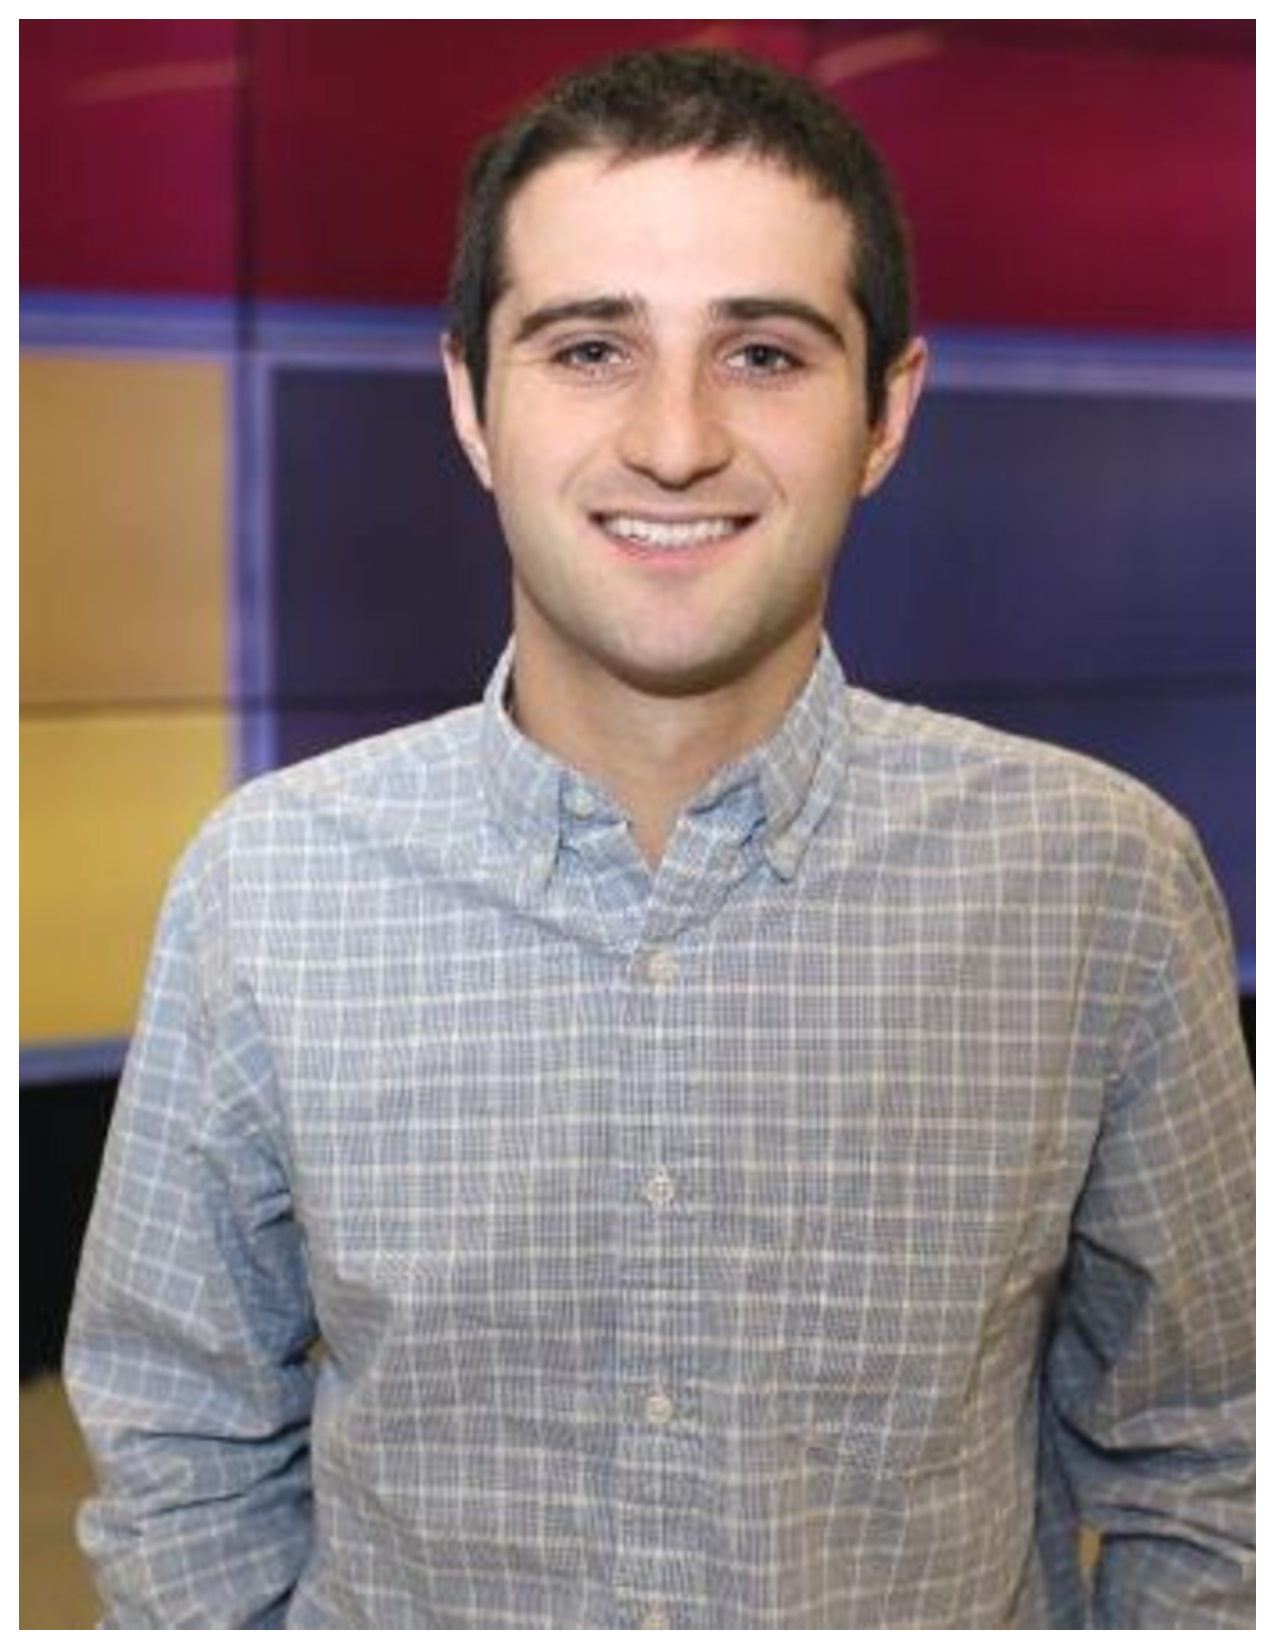
\includegraphics[width=0.25\columnwidth]{images/scott_mcclary}
  \end{wrapfigure}
  \noindent
  {\bfseries Scott McClary} received his BSc (Computer Science) and
  Minor (Mathematics) in May 2016 from Indiana University and will
  receive his MSc (Computer Science) in May 2017 from Indiana
  University. His research interests are within scientific application
  performance analysis on large-scale HPC systems. He will begin
  working as a Software Engineer with General Electric Digital in San
  Ramon, CA in July 2017.
\end{minipage}
\endgroup

\section*{} %used to create more spacing..
\section*{Work Breakdown}
The work on this project was distributed as follows between the
authors:
\begin{description}
\item[Scott McClary.] He completed all of the work for this paper
  including researching and testing Apache Airavata as well as
  composing this technology paper.
\end{description}

% Bibliography
\bibliography{references}
\end{document}

